\documentclass[../../main]{subfiles}

\renewcommand\thesection{\arabic{section}}


\begin{document}

\section{Shift Register System} \label{sec:}

Now let's move on to the controlling of \emph{actuators}. We can simply facilitate
this by using a handful of \emph{shift registers} as we did with multiplexer addressing
circuit. We have chosen to use \emph{74LS95}, a $4$ bit shift register that can be
directly driven by \esp as it is a \emph{74LS} series chip. Figure \ref{}

\begin{center}
    {\begin{minipage}[c] {0.42\textwidth}
        \centering

        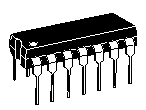
\includegraphics [
        ] {pics/74ls95_dip.pdf}
        \captionof{figure} {
            Dip package of \emph{74LS95}.
            \label{fig:74ls95Dip}
        }

        %\includegraphics [
        %    max width = \IGXMaxWidth,
        %    max height = \IGXMaxHeight,
        %    \IGXDefaultOptionalArgs,
        %] {../section_03/tikzpics/endAbsFiveBitShiftRegisterPinout.pdf}
        %\captionof{figure} {
        %    Pin diagram of \emph{74LS95}.
        %    \label{fig:74ls95PinDiagram}
        %}

        \includegraphics [
            max width = \IGXMaxWidth,
            max height = \IGXMaxHeight,
            \IGXDefaultOptionalArgs,
        ] {tikzpics/endAbsFourBitShiftRegisterPinout.pdf}
        \captionof{figure} {
            Pin diagram of \emph{74LS95}.
            \label{fig:74ls95PinDiagram}
        }

    \end{minipage}
    \hfill
    \begin{minipage}[c] {0.52\textwidth}

        \centering

        \begin{tabularx} {\linewidth} {
                *{1}{>{\centering\arraybackslash}m{0.3\linewidth}}
                *{1}{>{\centering\arraybackslash}m{0.7\linewidth}}
            }
            \toprule
            Pins & Remarks \\
            \midrule
            \texttt{PS A - PS E} & Preset lines (We are not using them). \\
            \texttt{Q A - Q E} & Parallel output lines. \\
            $\overline{\mbox{\texttt{MR}}}$ & Master reset (always tied high). \\
            \texttt{PE} & Preset enable (always tied low). \\
            \texttt{CP} & Clock pulse. \\
            \texttt{S} & Serial in. \\
            \bottomrule
        \end{tabularx}
        \captionof{table} {
            Relevant pins of \emph{74LS95}.
            \label{tbl:74ls95RelventPins}
        }

    \end{minipage}}

\end{center}

\end{document}
